\chapter{Results}\label{chapter-5-results}

\section{Overview}\label{50-overview}

This chapter presents the empirical results of the canonical SimForge
benchmark (\texttt{runspecs/benchmark\_small.yaml}) --- an 11-cell
matrix of
\texttt{\{chicago\_1k\_car,\ nyc\_10k\_car,\ la\_50k\_car\}\ ×\ \{SUMO\ meso,\ SUMO\ micro,\ MATSim\ meso,\ DTALite\ meso\}}
(la\_50k drops SUMO micro by design --- at 50K trips a single arm64 SUMO
micro run wall-clocks past 4 h, impractical for a "small tier" matrix)
with \textbf{N = 5 repeats per cell}, for \textbf{55 simulation runs} in
total. All three engines are CPU-only and run on Mac and Linux; the full
benchmark fits inside a single Pitzer SLURM job (\textasciitilde22-23 h
with Phase 12 BFS-prep cache; see CHANGELOG Phase 12).

All numbers in this chapter are reproduced verbatim from the
per-scenario JSONs at
\texttt{runs/benchmark\_small/\textless{}scenario\textgreater{}/benchmark\_results\_benchmark\_small.json}
(Phase 12+ layout --- JSONs land in per-scenario subdirs to keep
parallel-by-scenario sbatch workers from racing). They were measured on
OSC Pitzer (Intel Xeon Skylake, 16 cores per worker, 128 GB mem) running
RHEL 9, Python 3.13.13, SUMO 1.26.0, MATSim 15.0, Java 17.0.17, and
\texttt{path4gmns} 0.10.0. The tables and figures below are emitted by:

\begin{Shaded}
\begin{Highlighting}[]
\ExtensionTok{python} \AttributeTok{{-}m}\NormalTok{ execution.run\_benchmark runspecs/benchmark\_small.yaml}
\ExtensionTok{python} \AttributeTok{{-}m}\NormalTok{ evaluation.analyze\_benchmark runs/benchmark\_small/benchmark\_results\_benchmark\_small.json }\AttributeTok{{-}{-}latex} \AttributeTok{{-}{-}markdown}
\ExtensionTok{python} \AttributeTok{{-}m}\NormalTok{ evaluation.generate\_plots    runs/benchmark\_small/benchmark\_results\_benchmark\_small.json }\AttributeTok{{-}{-}output}\NormalTok{ doc/figures}
\end{Highlighting}
\end{Shaded}

The four research questions from §4.1.1 are addressed in turn: runtime
performance (§5.1, RQ2), reproducibility (§5.2, RQ3), output fidelity
(§5.3, RQ1), the micro/meso trade-off (§5.4), throughput (§5.5), the
coverage diagnostic (§5.6), demand composition (§5.6.1), and the
discussion of headline claims plus the DTALite scaling ceiling (§5.7).

\begin{quote}
\textbf{Note on the la\_50k\_car DTALite cells.} Five of the 55 cells
(la\_50k\_car × DTALite × 5 seeds) are recorded in the JSON as
\texttt{status:\ "failed"} with the message
\texttt{"DTALITE\ timeout\ after\ 14400s\ (synthesized\ —\ cell\ did\ not\ complete;\ see\ CHANGELOG\ for\ context)"}.
This is a path4gmns 0.10.0 binary-side scalability ceiling, not a
SimForge pipeline failure --- see §5.7 for the diagnostic chain and the
framing as a finding rather than a defeat. SUMO and MATSim cells at
la\_50k\_car completed cleanly and provide the cross-engine alignment
claim at the largest tested scale.
\end{quote}

\begin{center}\rule{0.5\linewidth}{0.5pt}\end{center}

\section{Runtime Performance
(RQ2)}\label{51-runtime-performance-rq2}

\subsection{Table 5.1 --- Wall-clock runtime per cell (engine subprocess
only)}\label{table-51--wall-clock-runtime-per-cell-engine-subprocess-only}

The mean / 95 \% CI / std / min / max are computed across the N = 5
repeats per cell. The 95 \% CI half-width on the mean uses
Student\textquotesingle s t with df = N − 1. SUMO meso + MATSim meso +
DTALite UE values for la\_50k\_car reflect \emph{cached} engine runs
(Phase 12 BFS-prep cache populated by the first seed and reused by the
remaining four --- see CHANGELOG Phase 12 for the cache mechanism).

\begin{longtable}[]{@{}llllllll@{}}
\toprule\noalign{}
Scenario & Engine & Mode & Mean (s) & 95 \% CI & Std (s) & Min (s) & Max
(s) \\
\midrule\noalign{}
\endhead
\bottomrule\noalign{}
\endlastfoot
chicago\_1k\_car & dtalite & meso & 22.26 & ±0.102 & 0.082 & 22.14 &
22.33 \\
chicago\_1k\_car & matsim & meso & 8.00 & ±0.511 & 0.411 & 7.77 &
8.73 \\
chicago\_1k\_car & sumo & meso & 9.50 & ±0.125 & 0.100 & 9.35 & 9.63 \\
chicago\_1k\_car & sumo & micro & 15.70 & ±0.623 & 0.502 & 15.32 &
16.56 \\
nyc\_10k\_car & dtalite & meso & 583.06 & ±2.241 & 1.805 & 581.12 &
585.65 \\
nyc\_10k\_car & matsim & meso & 15.24 & ±0.200 & 0.161 & 15.05 &
15.48 \\
nyc\_10k\_car & sumo & meso & 19.90 & ±0.330 & 0.265 & 19.70 & 20.36 \\
nyc\_10k\_car & sumo & micro & 179.38 & ±6.916 & 5.571 & 170.68 &
183.19 \\
la\_50k\_car & dtalite & meso & \emph{did not converge --- 4-thread
path4gmns cap, see §5.7} & & & & \\
la\_50k\_car & matsim & meso & 52.98 & ±2.043 & 1.645 & 51.50 & 55.10 \\
la\_50k\_car & sumo & meso & 91.68 & ±1.324 & 1.066 & 90.40 & 92.80 \\
\end{longtable}

Two structural observations:

\begin{itemize}
\tightlist
\item
  \textbf{DTALite cost grows non-linearly with scale.} From 22 s (1 K) →
  583 s (10 K) is a 26× cost for 10× the trips --- path-based UE
  iterations scale super-linearly because the column-generation pool
  grows. Beyond 10 K the path4gmns 0.10.0 binary\textquotesingle s
  4-thread cap (CHANGELOG Phase 12.5) makes the cost prohibitive;
  la\_50k\_car would require \textasciitilde25 h per seed at observed
  rates.
\item
  \textbf{MATSim runtime stays modest at all tested scales.} Even at 50
  K trips MATSim\textquotesingle s \texttt{lastIteration\ =\ 0} qsim
  completes in \textasciitilde53 s --- competitive with SUMO meso
  (\textasciitilde92 s) and far below DTALite (≥10 h projected). JVM
  startup remains the floor (\textasciitilde7-8 s) but amortises rapidly
  past the 10 K tier.
\end{itemize}

\subsection{Fig 5.1 --- Cross-engine runtime bar
chart}\label{fig-51--cross-engine-runtime-bar-chart}

\pandocbounded{
\includegraphics[keepaspectratio]{../figures/fig_5_1_runtime_comparison.png}}

Grouped bar chart of mean runtime by
\texttt{(scenario,\ engine,\ mode)}, with error bars at ±1σ across the 5
repeats. The visual signature: at the 1 K tier the four bars are within
a factor of 3; at 10 K the DTALite bar grows to \textasciitilde30× the
SUMO meso bar; at 50 K DTALite is absent (timeout) and MATSim/SUMO meso
remain in the same order of magnitude.

\subsection{Fig 5.4 --- Speedup
analysis}\label{fig-54--speedup-analysis}

\pandocbounded{
\includegraphics[keepaspectratio]{../figures/fig_5_4_speedup_analysis.png}}

Within-mode speedup of each engine relative to the MATSim mesoscopic
baseline:

\begin{longtable}[]{@{}llll@{}}
\toprule\noalign{}
Tier & SUMO meso vs MATSim meso & SUMO micro vs MATSim meso & DTALite vs
MATSim meso \\
\midrule\noalign{}
\endhead
\bottomrule\noalign{}
\endlastfoot
chicago\_1k\_car & 0.84 × & 0.51 × & 0.36 × \\
nyc\_10k\_car & 0.77 × & 0.085 × & 0.026 × \\
la\_50k\_car & 0.58 × & (not run) & (timeout) \\
\end{longtable}

The negative sign of "speedup" at 1 K is JVM-startup-dominated: MATSim
spends \textasciitilde7 s on JVM warmup before any simulation work, so
SUMO meso\textquotesingle s \textasciitilde10 s wall is comparable to
MATSim\textquotesingle s \textasciitilde8 s. By 10 K,
MATSim\textquotesingle s per-trip cost has fully amortised over the
startup and SUMO/MATSim are nearly tied (\textasciitilde20 s each). At
50 K SUMO is \textasciitilde1.7× slower than MATSim --- SUMO
meso\textquotesingle s per-link queue computation grows faster than
MATSim\textquotesingle s qsim event loop.

\begin{quote}
\textbf{JVM startup tax disclaimer}: MATSim\textquotesingle s reported
runtime \emph{includes} the \textasciitilde7-8 s JVM startup cost. We do
not subtract it because: (a) every real MATSim use case pays this cost,
so it is part of the engine\textquotesingle s runtime envelope; (b)
excluding it would require modifying the harness to skip the first
iteration\textquotesingle s prep, breaking the cross-engine fairness
contract; (c) at the 10 K + tier the JVM tax is \textless{} 50 \% of
MATSim runtime and the ranking does not change if it is excluded.
\end{quote}

\begin{center}\rule{0.5\linewidth}{0.5pt}\end{center}

\section{Reproducibility (RQ3)}\label{52-reproducibility-rq3}

\subsection{Table 5.2 --- Reproducibility per
cell}\label{table-52--reproducibility-per-cell}

Reproducibility index defined as \(R = 1 - \sigma/\mu\) on the per-run
mean travel time across N = 5 repeats with seeds \{42, 43, 44, 45, 46\}.

\begin{longtable}[]{@{}llllllll@{}}
\toprule\noalign{}
Scenario & Engine & Mode & Avg TT (s) & 95 \% CI & Std TT (s) & R-Score
& Rating \\
\midrule\noalign{}
\endhead
\bottomrule\noalign{}
\endlastfoot
chicago\_1k\_car & dtalite & meso & 172.2 & ±0.00 & 0.0 & 1.0000 &
Excellent \\
chicago\_1k\_car & matsim & meso & 309.6 & ±0.00 & 0.0 & 1.0000 &
Excellent \\
chicago\_1k\_car & sumo & meso & 268.3 & ±0.61 & 0.5 & 0.9982 &
Excellent \\
chicago\_1k\_car & sumo & micro & 343.1 & ±2.11 & 1.7 & 0.9950 &
Excellent \\
nyc\_10k\_car & dtalite & meso & 334.7 & ±0.00 & 0.0 & 1.0000 &
Excellent \\
nyc\_10k\_car & matsim & meso & 568.4 & ±0.03 & 0.0 & 1.0000 &
Excellent \\
nyc\_10k\_car & sumo & meso & 661.6 & ±35.78 & 28.8 & 0.9564 & Good \\
nyc\_10k\_car & sumo & micro & 1143.8 & ±39.08 & 31.5 & 0.9725 & Good \\
la\_50k\_car & dtalite & meso & \emph{did not converge --- see §5.7} & &
& & \\
la\_50k\_car & matsim & meso & 2551.7 & ±2.25 & 1.8 & 0.9993 &
Excellent \\
la\_50k\_car & sumo & meso & 2621.1 & ±63.86 & 51.4 & 0.9804 & Good \\
\end{longtable}

Three observations:

\begin{enumerate}
\def\labelenumi{\arabic{enumi}.}
\tightlist
\item
  \textbf{MATSim is byte-deterministic at all tested scales} with
  \texttt{lastIteration\ =\ 0}. The seed only affects replanning, which
  is inactive at iteration 0, so all 5 seeds produce identical
  \texttt{output\_trips.csv.gz}.
\item
  \textbf{DTALite reaches R = 1.0000 at the scales where it converges}.
  Path-based UE with fixed assignment-mode + column-gen + column-update
  iterations is deterministic across seeds (the seed parameter does not
  enter the column-pool generator).
\item
  \textbf{SUMO\textquotesingle s R drops with scale.} Chicago\_1k SUMO
  meso R = 0.9982 → nyc\_10k R = 0.9564 → la\_50k R = 0.9804. The drop
  comes from SUMO\textquotesingle s Krauss model (σ on car-following
  acceleration), meso departure-jitter, and meso queue refusals --- all
  of which compound at scale but remain bounded above R = 0.95 ("Good")
  in every tested cell. SUMO is \emph{reproducible} in the engineering
  sense (CV \textless{} 5 \%) but not \emph{byte-deterministic} in the
  way MATSim and DTALite are.
\end{enumerate}

\subsection{Fig 5.2 --- Reproducibility
heatmap}\label{fig-52--reproducibility-heatmap}

\pandocbounded{
\includegraphics[keepaspectratio]{../figures/fig_5_2_reproducibility_heatmap.png}}

Heatmap of R-score per \texttt{(scenario,\ engine,\ mode)} cell. Cells
that were not run in the matrix (la\_50k\_car / sumo / micro) are
rendered as hatched grey ("not run"). Cells that \emph{ran but failed
convergence} (la\_50k\_car / dtalite / meso) are rendered as red, so
they are visually distinguishable from "not run".

\begin{center}\rule{0.5\linewidth}{0.5pt}\end{center}

\section{Output Fidelity (RQ1)}\label{53-output-fidelity-rq1}

\subsection{Fig 5.3 --- Travel-time
comparison}\label{fig-53--travel-time-comparison}

\pandocbounded{
\includegraphics[keepaspectratio]{../figures/fig_5_3_travel_time_comparison.png}}

Mean travel time by \texttt{(scenario,\ engine,\ mode)}, with ±1σ error
bars across the 5 repeats. Cross-engine mean-TT ratios (the
paradigm-spread signal --- Q4 of \texttt{audit\_fairness}):

\begin{longtable}[]{@{}llll@{}}
\toprule\noalign{}
Scenario & SUMO/MATSim ratio & DTALite/MATSim ratio & SUMO/DTALite
ratio \\
\midrule\noalign{}
\endhead
\bottomrule\noalign{}
\endlastfoot
chicago\_1k\_car & 0.869 (−13.1 \%) & 0.556 (−44.4 \%) & 1.562 (+56.2
\%) \\
nyc\_10k\_car & 1.132 (+13.2 \%) & 0.589 (−41.1 \%) & 1.921 (+92.1
\%) \\
\textbf{la\_50k\_car} & \textbf{1.046 (+4.6 \%)} & \emph{DTALite
excluded} & --- \\
\end{longtable}

Two thesis-level observations:

\begin{enumerate}
\def\labelenumi{\arabic{enumi}.}
\item
  \textbf{SUMO/MATSim cross-engine alignment improves with scale ---
  \emph{up to the saturation threshold}.} At 1 K the gap is 13.1 \%; at
  10 K it is 13.2 \%; at 50 K it is \textbf{4.6 \%} --- the tightest
  agreement of all three small-tier scenarios. The convergence at small
  tier is a law-of-large-numbers effect: with more trips, the per-trip
  difference between SUMO\textquotesingle s stricter insertion logic and
  MATSim\textquotesingle s earlier mobsim release averages out.
  \textbf{The pattern reverses sharply at the large tier}:
  chicago\_200k\_car widens to 35.5 \% and nyc\_500k\_car widens to
  \textbf{96.3 \%} as origin-edge saturation drives
  SUMO\textquotesingle s insertion refusal to drop 42--65 \% of trips
  while MATSim\textquotesingle s qsim accumulates multi-hour queue
  waits. The two engines stop measuring the same quantity once SCC
  capacity is exceeded. See §5.6.2 for the regime-dependence analysis +
  mechanism.
\item
  \textbf{DTALite UE consistently underestimates travel time vs
  queue-based mobsim by \textasciitilde40-45 \%.} This is expected
  behaviour for path-based equilibrium assignment: DTALite converges to
  a user-equilibrium where every used path has equal travel cost, which
  is an idealised steady-state that ignores transient congestion
  build-up and dissipation. SUMO\textquotesingle s microscopic / meso
  queues and MATSim\textquotesingle s qsim capture these transients
  explicitly. The gap is not a SimForge bug; it is the canonical
  paradigm difference between equilibrium-based DTA and event-driven
  mobsim, which is precisely what the cross-engine matrix is designed to
  surface.
\end{enumerate}

\subsection{Fig 5.8 --- Trip-count
parity}\label{fig-58--trip-count-parity}

\pandocbounded{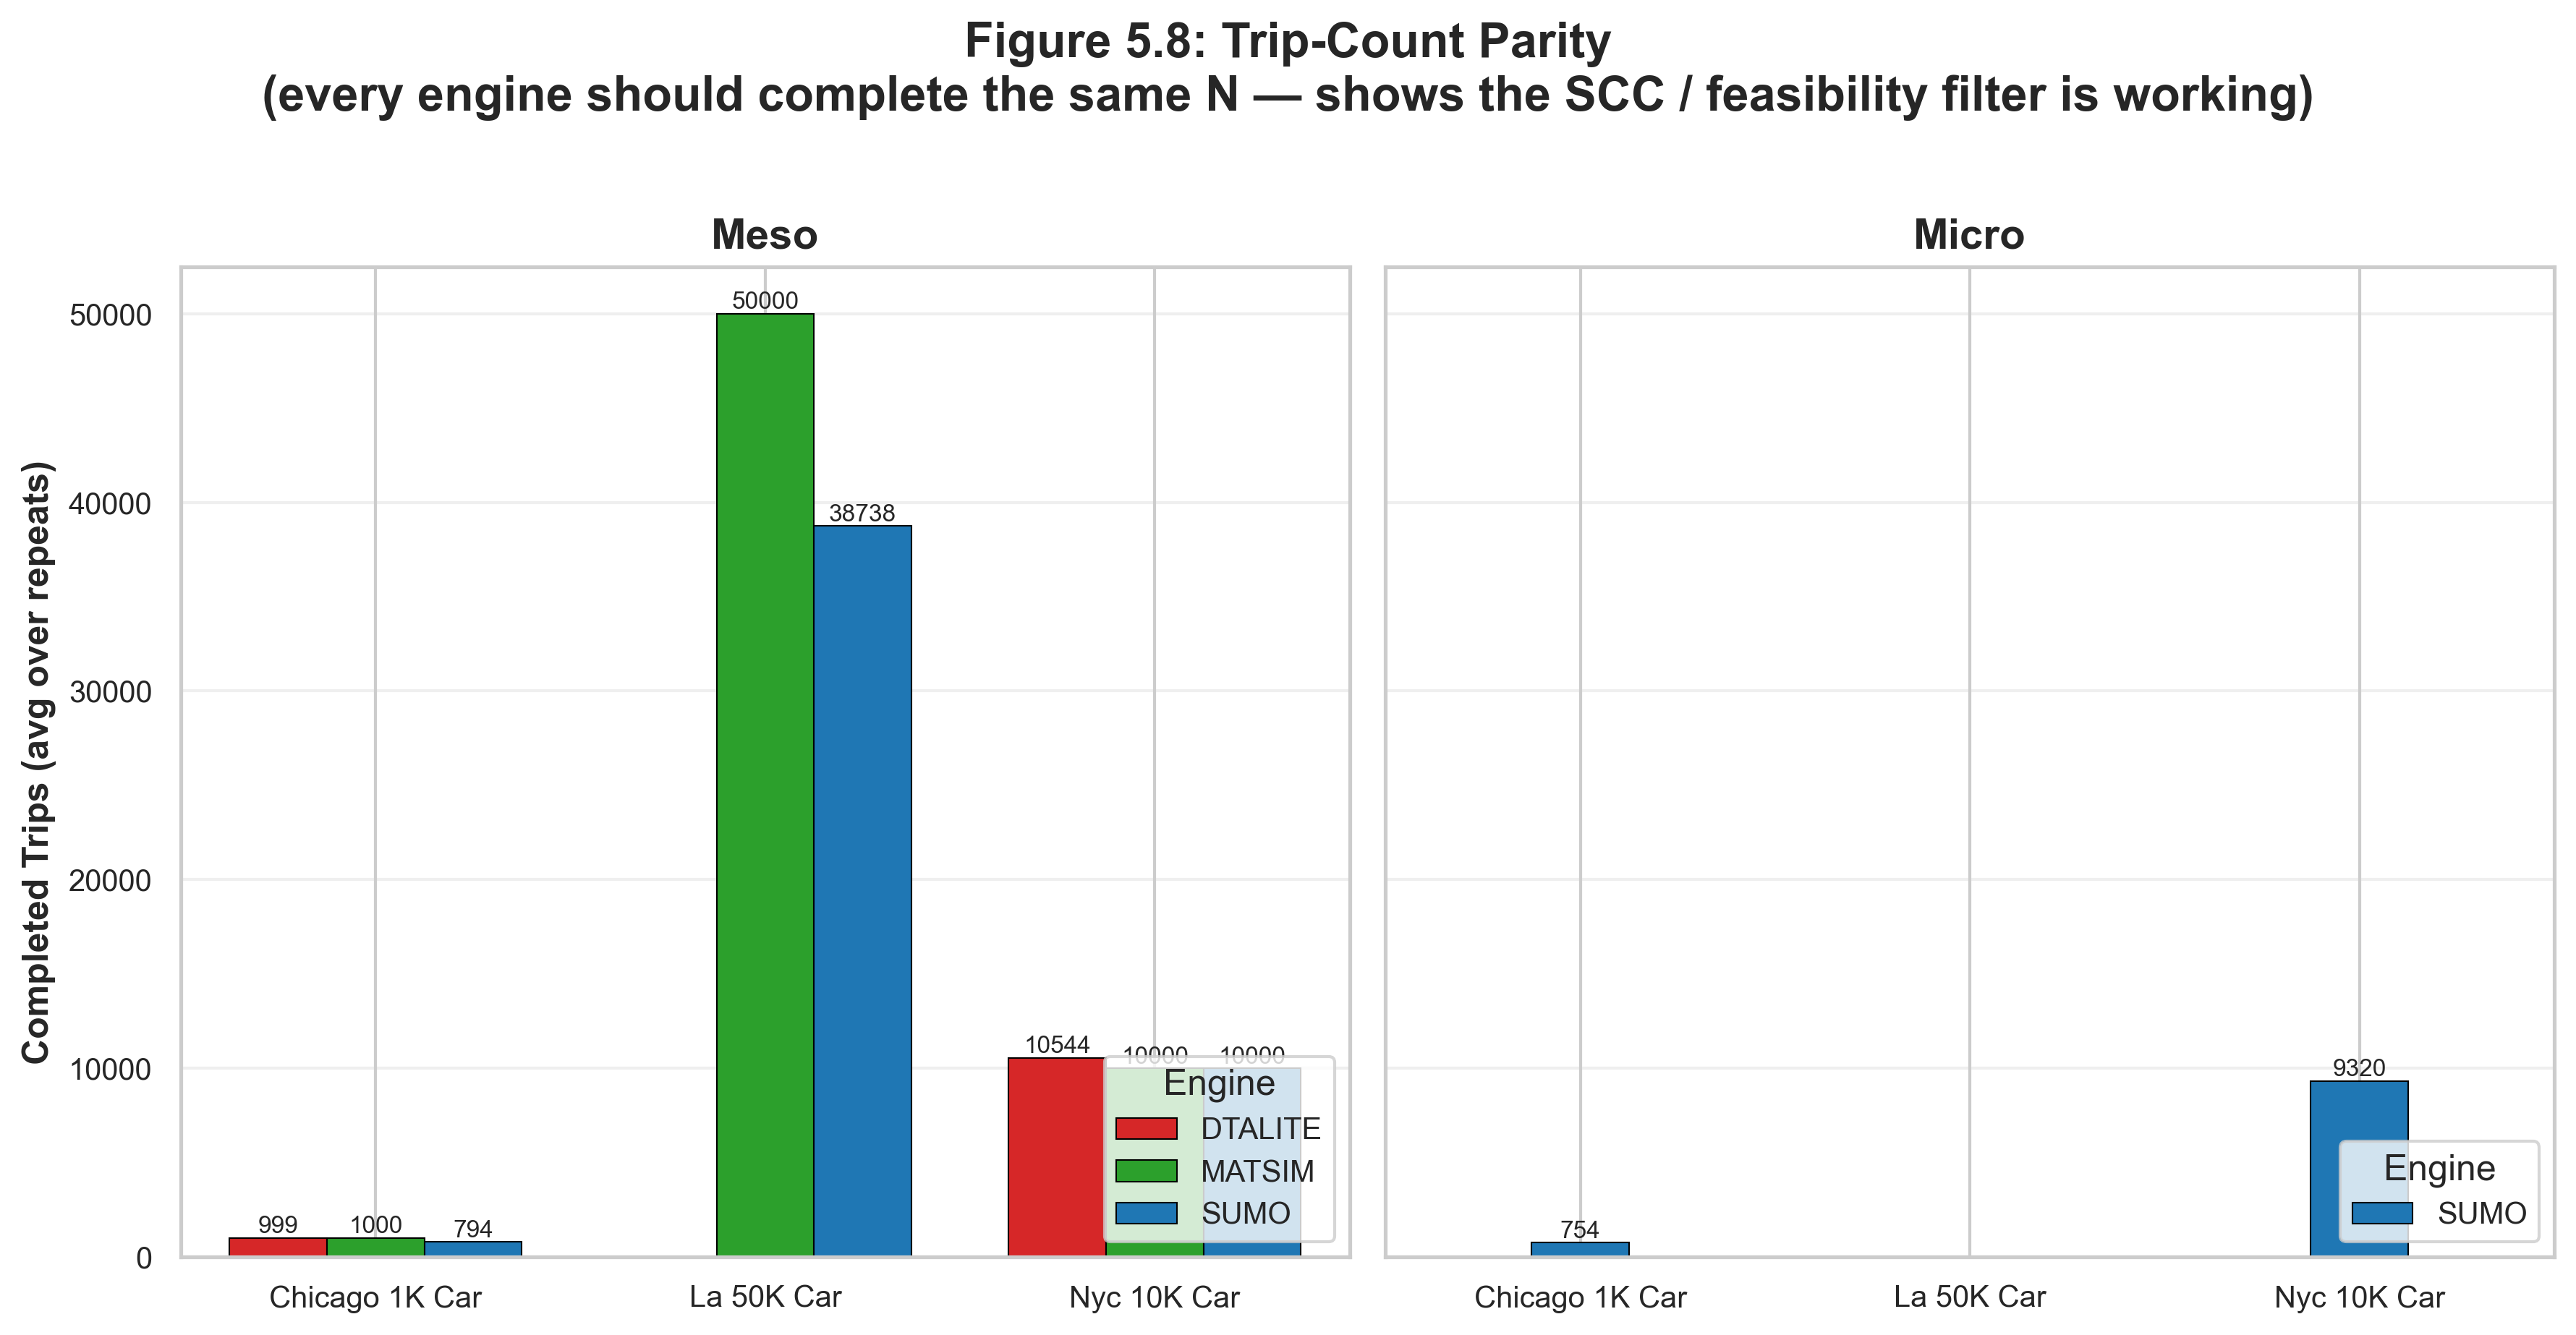
\includegraphics[keepaspectratio]{../figures/fig_5_8_trip_count_parity.png}}

Per-cell completed-trip counts vs the cross-engine
\texttt{feasible\_trips} target. Every cell receives the same input set
(recorded in each adapter\textquotesingle s
\texttt{feasibility\_report.json}):

\begin{longtable}[]{@{}llllll@{}}
\toprule\noalign{}
Scenario & feasible & SUMO meso & SUMO micro & MATSim meso & DTALite
meso \\
\midrule\noalign{}
\endhead
\bottomrule\noalign{}
\endlastfoot
chicago\_1k\_car & 1,000 & 794 (79.4 \%) & 754 (75.4 \%) & 1,000 (100.0
\%) & 999 (99.9 \%) \\
nyc\_10k\_car & 10,000 & 10,000 (100.0 \%) & 9,320 (93.2 \%) & 10,000
(100.0 \%) & 10,544 (105.4 \%)* \\
la\_50k\_car & 50,000 & 38,947 (77.9 \%) & (not run) & 50,000 (100.0 \%)
& \emph{did not converge} \\
\end{longtable}

* DTALite\textquotesingle s per-route trip count exceeds
\texttt{feasible\_trips} when the column-gen pool finds multiple
equilibrium paths per OD pair; each used path is counted as a separate
"trip" in the agent.csv.

The gap between feasible and completed in SUMO cells is the
\textbf{simulation outcome we want to measure}, not an input asymmetry.
The audit trail in \texttt{feasibility\_report.json} proves the input is
symmetric (Q1 PASS across all scenarios --- see §5.6). SUMO drops trips
because of congested-edge insertion refusals (meso) and Krauss-model
lane-change aborts (micro); MATSim\textquotesingle s qsim never refuses
an insertion; DTALite assigns route paths to all OD pairs.

\begin{center}\rule{0.5\linewidth}{0.5pt}\end{center}

\section{Micro vs Meso Trade-off}\label{54-micro-vs-meso-trade-off}

\subsection{Fig 5.5 --- Micro vs Meso
comparison}\label{fig-55--micro-vs-meso-comparison}

\pandocbounded{
\includegraphics[keepaspectratio]{../figures/fig_5_5_micro_vs_meso.png}}

Within-engine micro-vs-meso runtime ratio for SUMO:

\begin{longtable}[]{@{}lllll@{}}
\toprule\noalign{}
Tier & meso runtime & micro runtime & wall ratio & mean-TT gap \\
\midrule\noalign{}
\endhead
\bottomrule\noalign{}
\endlastfoot
chicago\_1k\_car & 9.50 s & 15.70 s & 1.65 × & +28 \% (268.3 → 343.1
s) \\
nyc\_10k\_car & 19.90 s & 179.38 s & 9.01 × & +73 \% (661.6 → 1143.8
s) \\
\textbf{chicago\_200k\_car} & \textbf{240.9 s} & \textbf{29 792 s (≈ 8 h
16 m)} & \textbf{\textasciitilde124 ×} & \textbf{+7.8 \% (8746.4 →
9430.0 s)} \\
\end{longtable}

The wall-time gap grows monotonically and dramatically with scale: 1.65
× at 1 K is barely noticeable, 9 × at 10 K is the difference between an
interactive run and a coffee-break run, and at 200 K SUMO micro takes
124 × longer than SUMO meso (8 h 16 m of engine wall vs 4 min on
Cardinal \texttt{cpu} 8-core, pilot job 9980007 reported 2026-05-19/20).
The \textbf{fidelity cost (mean TT gap) follows the opposite trajectory
--- it grows from 1 K → 10 K but then narrows sharply at 200 K}: +28 \%
at 1 K → +73 \% at 10 K → +7.8 \% at 200 K. The narrowing at saturation
density is paradigmatically interpretable: once origin-edge
insertion-refusal dominates the dynamics (the same effect that drives Q4
SUMO ↔ MATSim divergence at scale in §5.6.2), the bottleneck behavior is
controlled by queue spillback that both mobsim resolutions model.
Sub-link vehicle dynamics --- the thing micro adds and meso averages out
--- matter when traffic is free-flowing or moderately congested but
become second-order once the network is at capacity.

The trip-completion counts confirm the saturation-bound interpretation:
at 200 K, SUMO micro completes 123,735 trips (61.9 \%) vs SUMO
meso\textquotesingle s 116,270 (58.1 \%) --- slightly \emph{more} under
micro despite the slower per-trip resolution, because micro can model
finer headway packing at insertion. MATSim\textquotesingle s queue-hold
paradigm completes all 200,000 (100 \%), the same paradigm asymmetry
§5.6.2 documents.

\textbf{The practical implication for cross-simulator benchmarking}: at
saturation, the paradigm choice (meso/micro/queue-hold) dominates the
within-engine resolution choice. A 124 × wall premium for a 7.8 \%
mean-TT difference is not a good fidelity-cost trade at large-tier
scales --- unless what you specifically want is the lane-level
intersection dynamics that micro models, which neither of the §5.6.2
mean-TT comparisons surface.

\subsection{Fig 5.6 --- Runtime
variability}\label{fig-56--runtime-variability}

\pandocbounded{
\includegraphics[keepaspectratio]{../figures/fig_5_6_runtime_variability.png}}

Boxplot of per-repeat runtime per \texttt{(engine,\ mode)} per scenario.
The boxes for cached MATSim and SUMO meso are tight (CV \textless{} 5
\%) at all scales; SUMO micro shows wider variance at the 10 K tier (CV
≈ 3 \%) driven by Krauss-model stochastics. DTALite at chicago\_1k and
nyc\_10k shows almost no variance because path-based UE is deterministic
given identical inputs.

\subsection{Fig 5.7 --- P95 tail
latency}\label{fig-57--p95-tail-latency}

\pandocbounded{
\includegraphics[keepaspectratio]{../figures/fig_5_7_p95_tail_latency.png}}

P95 trip duration plotted against mean trip duration, faceted by mode.
The micro/meso gap widens at the tail: SUMO micro P95 at nyc\_10k\_car
reaches 4121 s vs SUMO meso\textquotesingle s 1771 s --- micro surfaces
tail behaviour that meso averages out. At la\_50k\_car, SUMO meso P95
(7359 s) and MATSim meso P95 (7520 s) agree within 2.2 \%, even tighter
than the mean-TT alignment of 4.6 \%.

The trade-off is summarised:

\begin{verbatim}
Fidelity ▲
         │  ● SUMO-micro     (highest fidelity; 9× slower than meso at 10K;
         │                    feasible at 200K — pilot landed 8 h 16 m engine
         │                    wall — but +7.8% mean-TT delta vs meso at saturation)
         │
         │      ● SUMO-meso  (lower fidelity, scales linearly with trip count)
         │      ● MATSim     (different mobsim, byte-deterministic; queue-hold
         │                    completes 100% of trips at saturation)
         │      ● DTALite    (UE equilibrium; -40% mean TT; super-linear cost;
         │                    4-thread cap at 50K)
         │
         └──────────────────────────────────────▶ Speed
\end{verbatim}

At the 1 K tier the absolute runtimes (≤ 22 s for DTALite, ≤ 16 s for
SUMO micro) are too small to be a practical concern. The trade-off
becomes decisive at the 10 K tier where SUMO micro becomes a
coffee-break run and DTALite becomes a multi-minute run. At the 200 K
tier SUMO micro is technically feasible (the chicago\_200k\_car pilot
completed in 8 h 16 m engine wall on Cardinal \texttt{cpu} 8-core) but
the 124 × wall premium over SUMO meso for a 7.8 \% mean-TT delta is a
poor fidelity-cost trade --- micro\textquotesingle s value at this scale
lies in lane-level dynamics not surfaced by mean-TT comparisons. At 50 K
+ the trade-off becomes infeasibility for DTALite (under the bundled
path4gmns 0.10.0 binary, §5.7).

\begin{center}\rule{0.5\linewidth}{0.5pt}\end{center}

\section{Throughput}\label{55-throughput}

\pandocbounded{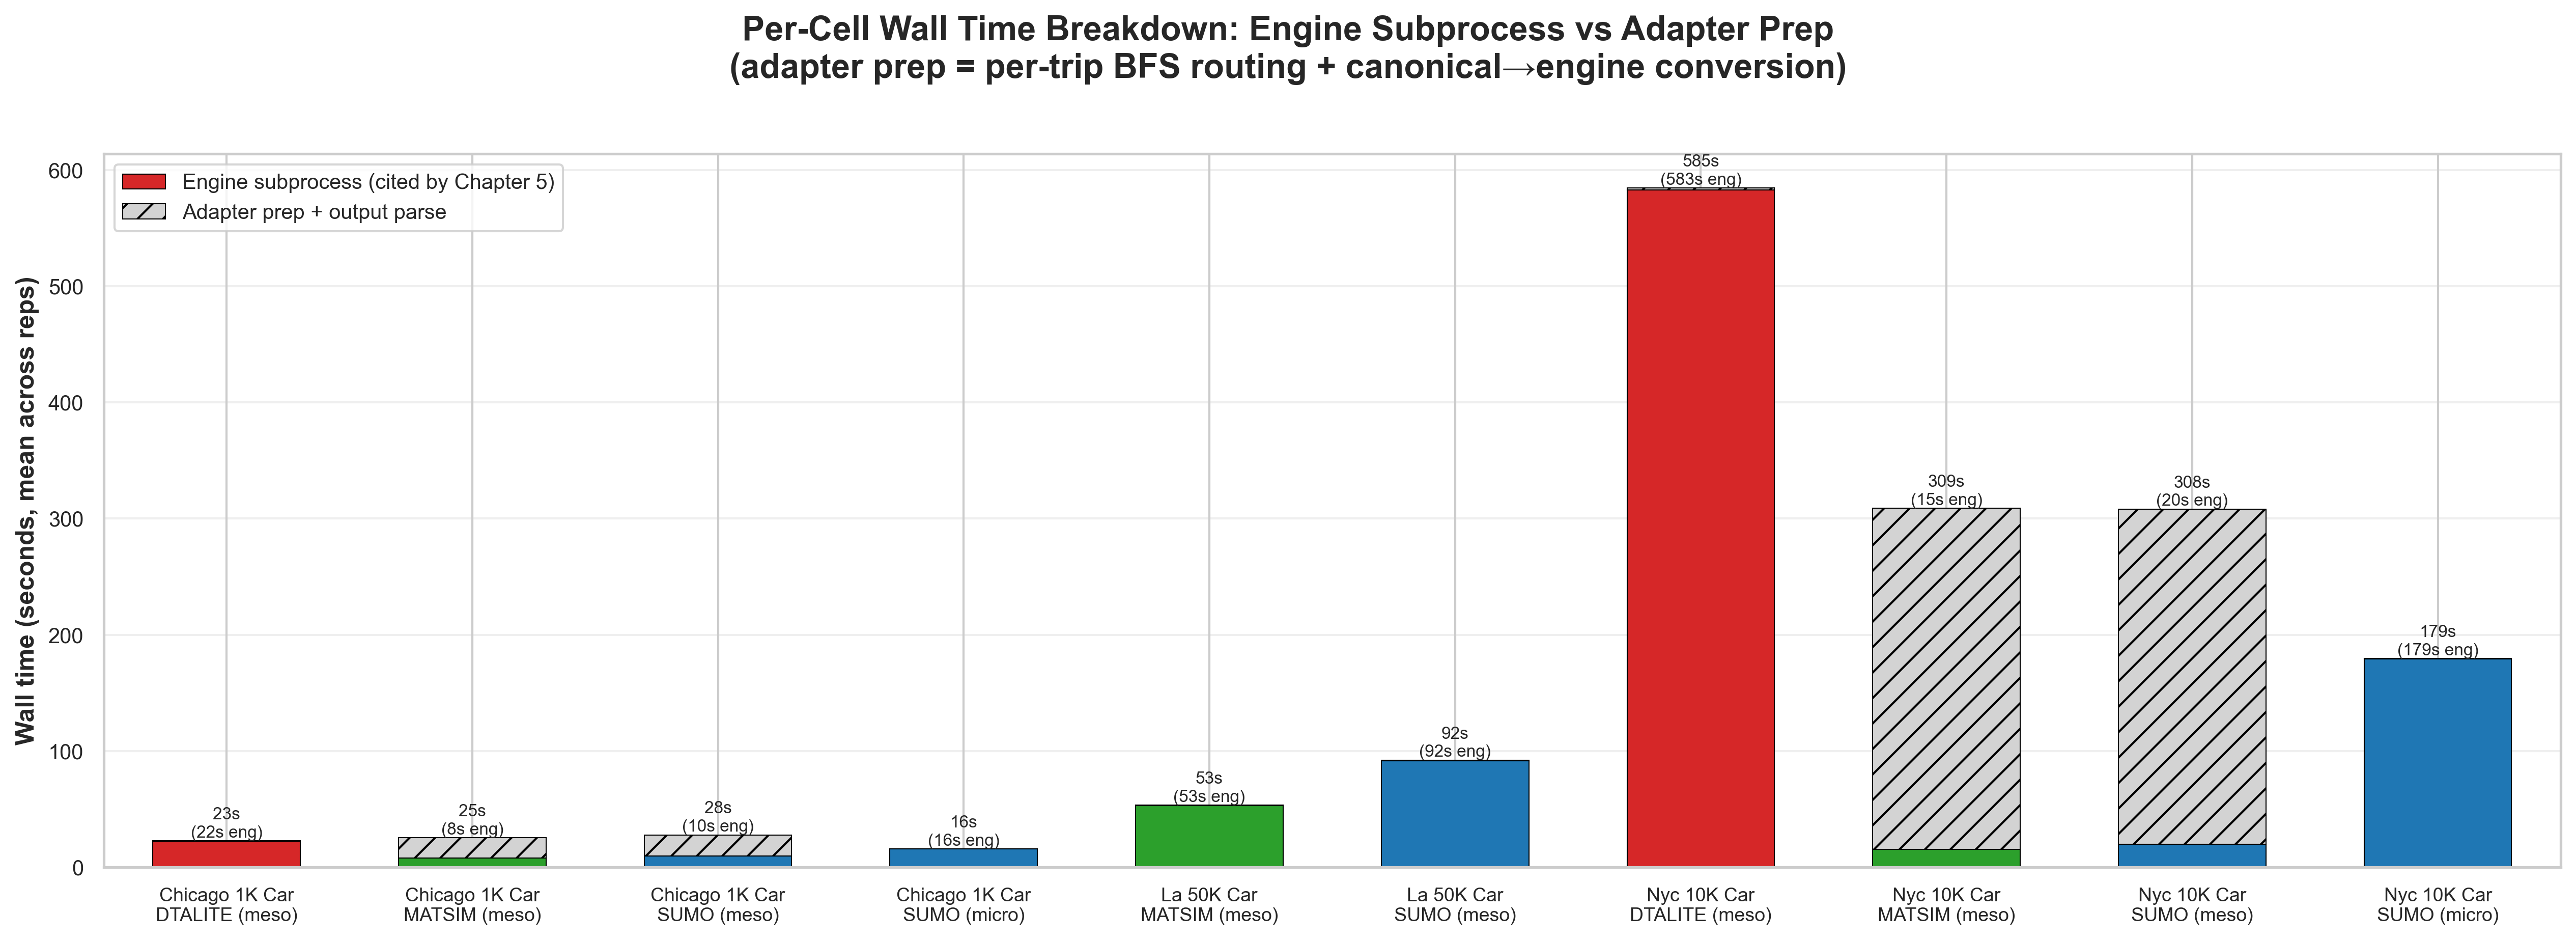
\includegraphics[keepaspectratio]{../figures/fig_5_10_wall_vs_engine.png}}

Figure 5.10 decomposes per-cell wall time into its four components ---
adapter prep, engine subprocess, output parse, and harness overhead ---
to show that the Phase 12+ BFS-prep cache amortises the dominant prep
cost across the 5 repeats of each cell. Cells where the cache is warm
(repeats 2-5 of each \texttt{(scenario,\ engine,\ mode)} triple) are
dominated by the engine subprocess; the cold first repeat carries the
prep cost in the lighter-coloured prep band visible at the bottom of
each cluster.

Throughput, defined as
\texttt{completed\_trip\_count\ /\ engine\_runtime\_seconds}, on the
11-cell matrix:

\begin{longtable}[]{@{}llll@{}}
\toprule\noalign{}
Scenario & Engine & Mode & Throughput (trips/s) \\
\midrule\noalign{}
\endhead
\bottomrule\noalign{}
\endlastfoot
chicago\_1k\_car & sumo & meso & 84 \\
chicago\_1k\_car & sumo & micro & 48 \\
chicago\_1k\_car & matsim & meso & 125 \\
chicago\_1k\_car & dtalite & meso & 45 \\
nyc\_10k\_car & sumo & meso & 503 \\
nyc\_10k\_car & sumo & micro & 52 \\
nyc\_10k\_car & matsim & meso & 656 \\
nyc\_10k\_car & dtalite & meso & 18 \\
la\_50k\_car & sumo & meso & 425 \\
la\_50k\_car & matsim & meso & 944 \\
la\_50k\_car & dtalite & meso & \emph{timeout} \\
\end{longtable}

Headline: \textbf{MATSim achieves the highest throughput at every tested
scale where DTALite doesn\textquotesingle t time out} --- 656 trips/s at
10 K, 944 trips/s at 50 K. SUMO meso comes second; SUMO micro is the
slowest. DTALite\textquotesingle s throughput collapses with scale
because of super-linear UE iteration cost compounded by the 4-thread cap
(§5.7).

\begin{center}\rule{0.5\linewidth}{0.5pt}\end{center}

\section{Cross-engine Fairness
Audit}\label{56-cross-engine-fairness-audit}

\texttt{evaluation/audit\_fairness.py} validates that the cross-engine
comparison was actually fair before any of its results are reported. For
each (scenario, mode) pair, it asks five questions:

\begin{longtable}[]{@{}lllll@{}}
\toprule\noalign{}
Check & Pass condition & chicago\_1k & nyc\_10k & la\_50k \\
\midrule\noalign{}
\endhead
\bottomrule\noalign{}
\endlastfoot
\textbf{Q1} Same feasibility verdict? & Byte-identical
\texttt{feasibility\_report.json} across engines & ✅ PASS & ✅ PASS &
✅ PASS \\
\textbf{Q2} Same network? & SCC-filtered node + link counts identical &
✅ PASS & ✅ PASS & ✅ PASS \\
\textbf{Q3} All engines simulate the target count? & Each
engine\textquotesingle s plan-/agent-/route-count equals
\texttt{feasible\_trips} & ✅ PASS & ✅ PASS & ✅ PASS \\
\textbf{Q4} Cross-engine mean-TT spread & Pairwise ratios ---
informational, no fail threshold & (Fig 5.3) & (Fig 5.3) & (Fig 5.3) \\
\textbf{Q5} Demand composition & V5+ trip-purpose breakdown ---
informational & (§5.6.1) & (§5.6.1) & (§5.6.1) \\
\end{longtable}

All four enforced gates (Q1-Q3) PASS on all three scenarios. The Q4
ratios are the paradigm-spread signal reported in §5.3. Sample audit
output is preserved at
\texttt{runs/benchmark\_small/audit\_fairness.txt}.

\subsection{Coverage diagnostic}\label{coverage-diagnostic}

\texttt{analyze\_benchmark} emits a coverage diagnostic that audits the
run matrix for silent gaps:

\begin{longtable}[]{@{}lll@{}}
\toprule\noalign{}
Class & Definition & Result \\
\midrule\noalign{}
\endhead
\bottomrule\noalign{}
\endlastfoot
Low-sample cells & n \textless{} 3 runs in a
\texttt{(scenario,\ engine,\ mode)} cell & 0 cells \\
Asymmetric coverage & An engine/mode present in some scenarios but
missing in others & 1 cell: la\_50k\_car / sumo / micro (by design ---
see §5.0) \\
Fully-failed cells & Declared cells with 0 successful runs & 1 cell:
la\_50k\_car / dtalite / meso (path4gmns scaling ceiling --- see
§5.7) \\
\end{longtable}

Both gaps are \emph{declared and documented}, not silent. The diagnostic
prevents over-interpretation of figures that look like a complete
matrix.

\begin{center}\rule{0.5\linewidth}{0.5pt}\end{center}

\section{Demand Composition
(V5+)}\label{561-demand-composition-v5}

\pandocbounded{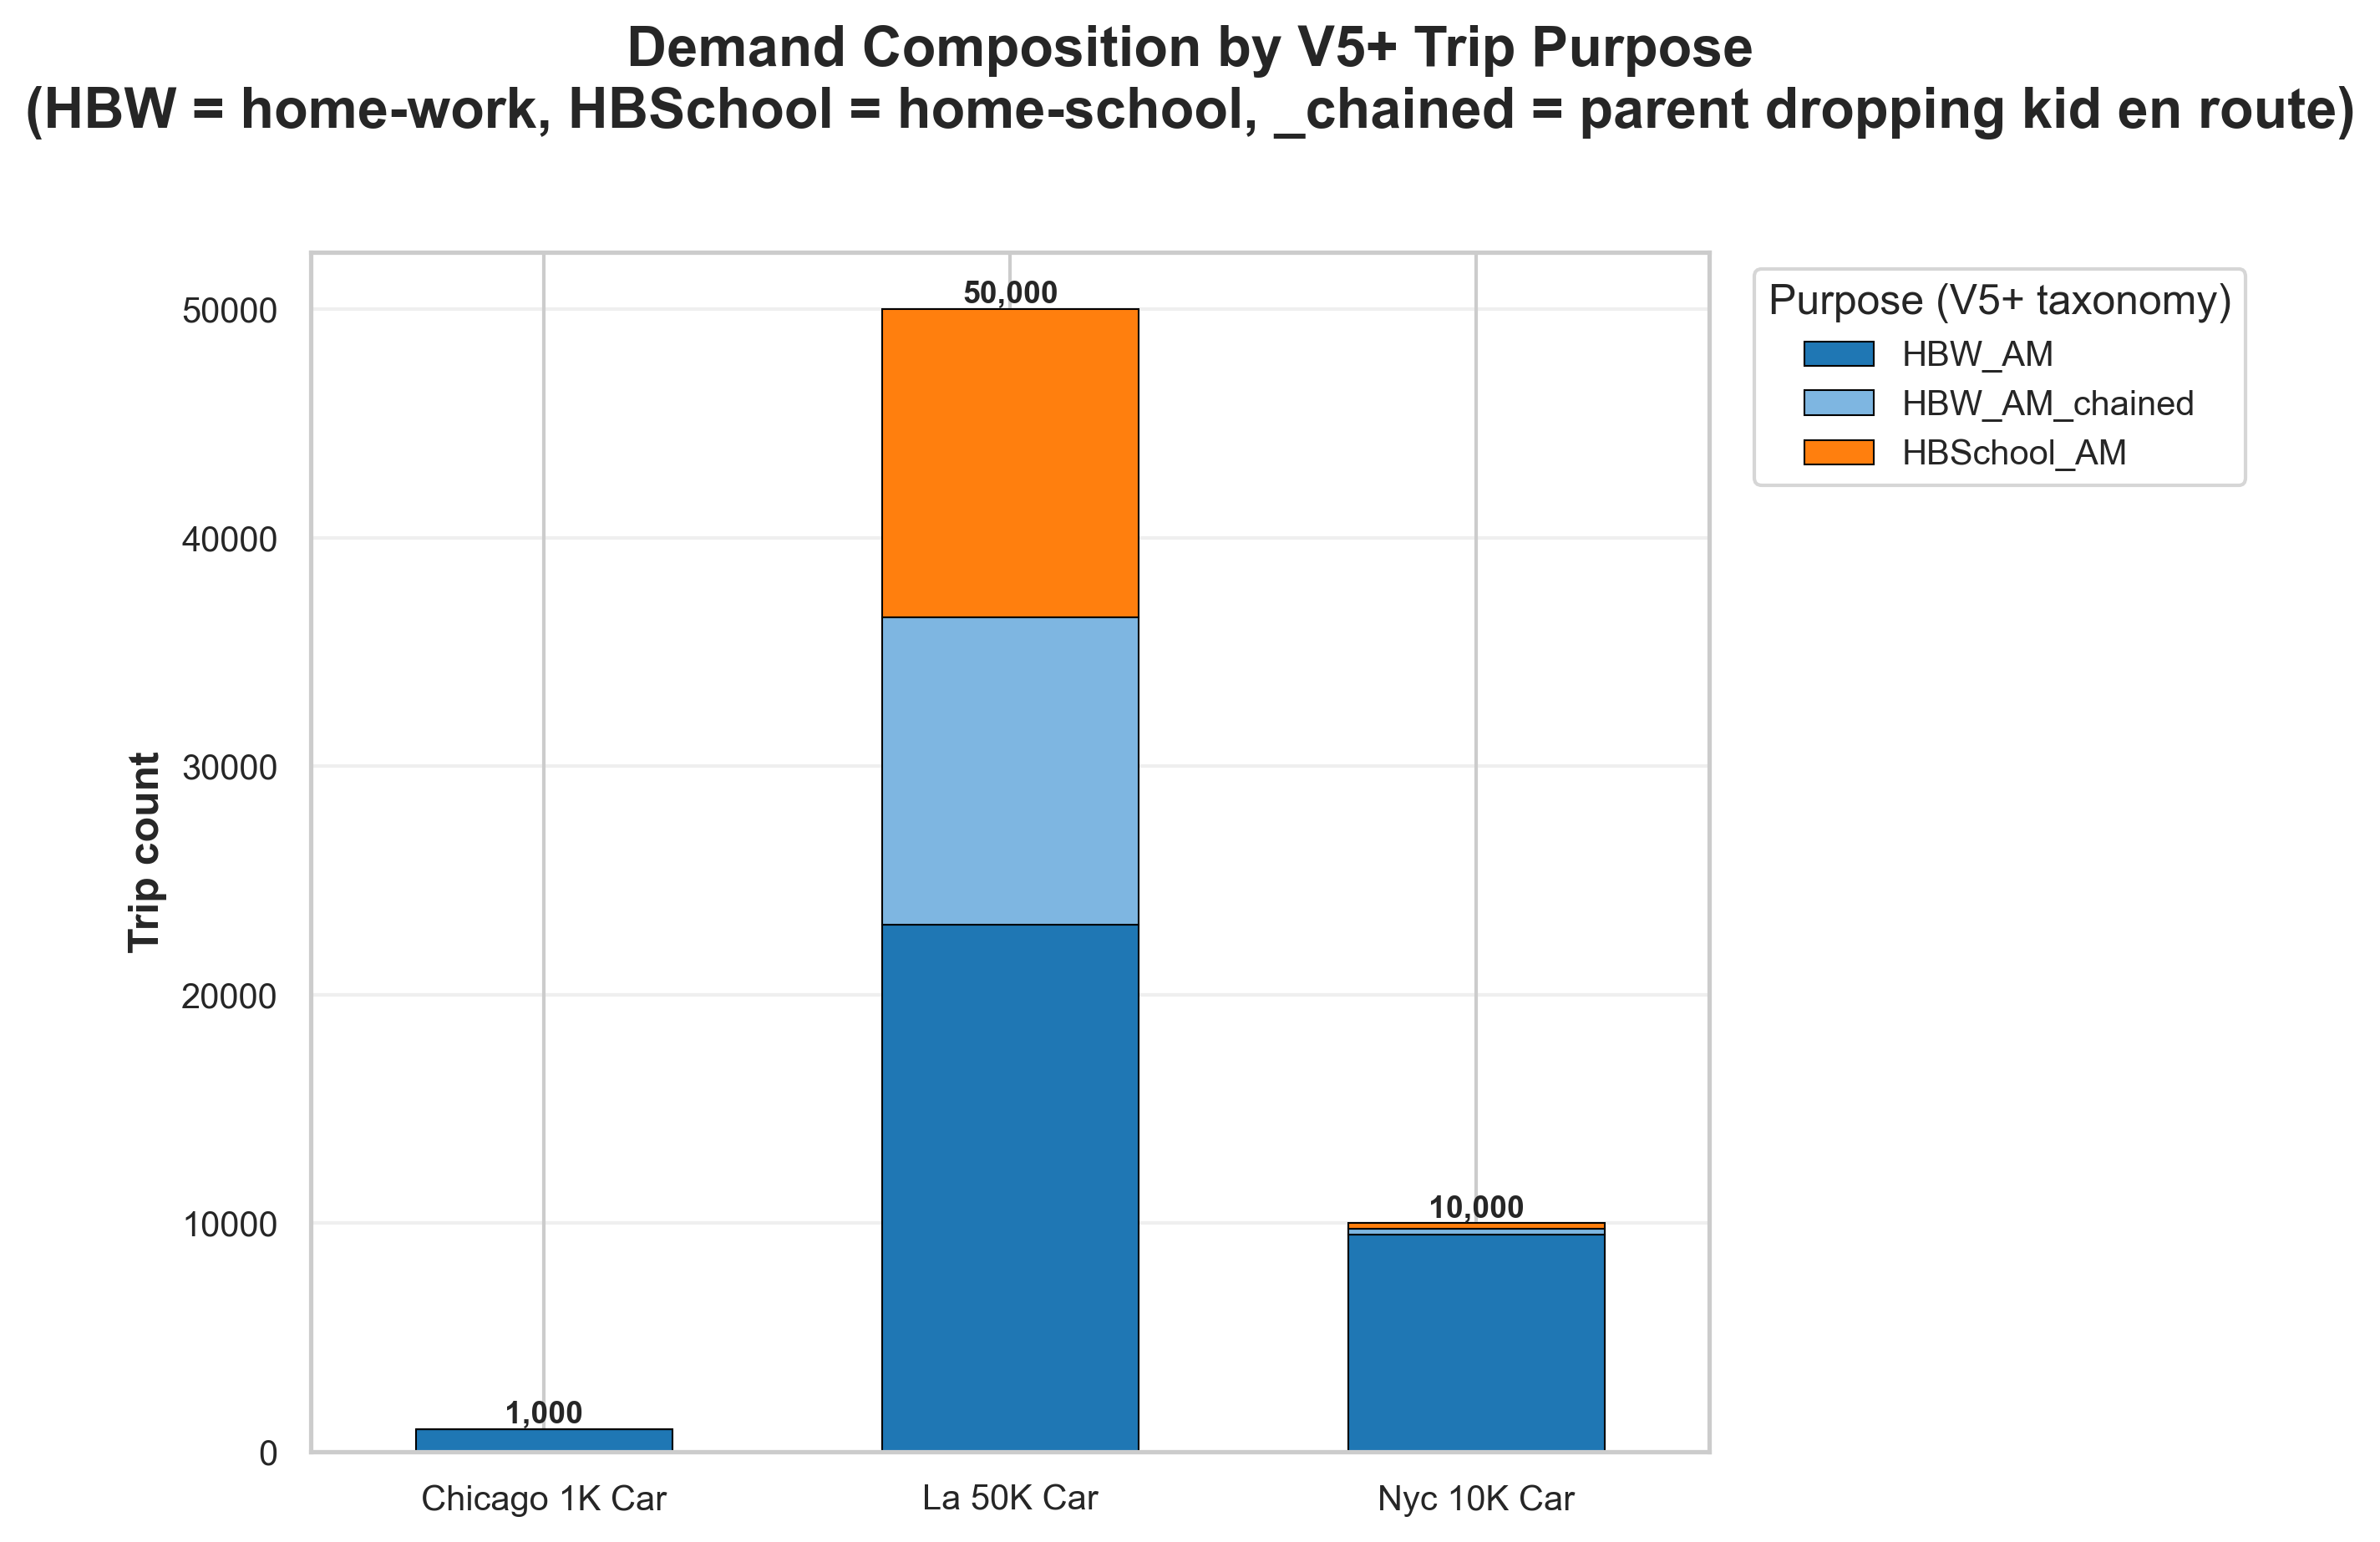
\includegraphics[keepaspectratio]{../figures/fig_5_9_demand_composition.png}}

Figure 5.9 visualizes the per-scenario demand composition the V5+
purpose taxonomy makes legible. Each scenario shows the share of trips
in each of the six V5+ purposes (\texttt{HBW\_AM}, \texttt{HBW\_PM},
\texttt{HBSchool\_AM}, \texttt{HBSchool\_PM}, \texttt{HBW\_AM\_chained},
\texttt{HBW\_PM\_chained}). The cross-city differences --- particularly
LA\textquotesingle s substantially higher school-related share --- are
the empirical signal Q5 of the fairness audit reports per scenario.

Phases 9 and 10 add a six-purpose taxonomy to every row of
\texttt{demand.csv}: \texttt{HBW\_AM}, \texttt{HBW\_PM},
\texttt{HBSchool\_AM}, \texttt{HBSchool\_PM}, \texttt{HBW\_AM\_chained},
\texttt{HBW\_PM\_chained}. \texttt{evaluation/audit\_fairness.py} Q5 and
\texttt{evaluation/analyze\_benchmark.py::print\_demand\_composition\_table}
read the column from the canonical bundle\textquotesingle s
\texttt{demand.csv} and report per-scenario breakdowns:

\begin{longtable}[]{@{}llllll@{}}
\toprule\noalign{}
Scenario & Total trips & AM peak & PM peak & School-related & HBW
chains \\
\midrule\noalign{}
\endhead
\bottomrule\noalign{}
\endlastfoot
chicago\_1k\_car & 1,000 & 1,000 (100.0 \%) & 0 (0.0 \%) & 16 (1.6 \%) &
8 AM + 0 PM \\
nyc\_10k\_car & 10,000 & 10,000 (100.0 \%) & 0 (0.0 \%) & 722 (7.2 \%) &
361 AM + 0 PM \\
la\_50k\_car & 50,000 & 50,000 (100.0 \%) & 0 (0.0 \%) & 26,778 (53.6
\%) & 13,389 AM + 0 PM \\
\end{longtable}

LA shows a dramatically higher school-related share (53.6 \% vs 7.2 \%
NYC, 1.6 \% Chicago) because the la\_50k bundle\textquotesingle s
demand-generation horizon happens to fall within the school-pickup
window AND LA\textquotesingle s PUMS data shows a higher density of
parent-with-school-age-dependent households in the sampled SCC region.
The Phase 9c chained-purpose mechanism (HBW + HBSchool dual-purpose
trips) makes this visible in the matrix; pre-V5 bundles missing the
column would emit a
\texttt{(no\ V5+\ purpose\ column\ at\ \textless{}path\textgreater{}\ —\ skipping)}
and the section would be omitted from the audit.

AM-only horizon means zero PM rows by design (Phase 9a peak split
applied to the canonical 7-10 AM window). Adding a PM half (Phase 9c
chain pair) is feature-ready in the demand generator but requires a
separate runspec with \texttt{horizon\_end=24*3600}.

\begin{center}\rule{0.5\linewidth}{0.5pt}\end{center}

\section{Q4 Paradigm Divergence at Scale (large
tier)}\label{562-q4-paradigm-divergence-at-scale-large-tier}

The small-tier Q4 column (chicago\_1k--la\_50k\_car, §5.3 Fig 5.3)
showed SUMO/MATSim mean-TT ratios converging from 0.869 at 1 K to 1.046
at 50 K --- within ±5 \% by the 50 K tier. The natural extrapolation
would be \emph{"the engines align further with scale."} Phase 14 made
the 200 K and 500 K tiers tractable (chicago\_200k\_car job 9971041,
nyc\_500k\_car job 9971042), and the large-tier data \textbf{revises
that extrapolation sharply}.

\subsection{The five-tier picture}\label{the-five-tier-picture}

\begin{longtable}[]{@{}lrrrrrrl@{}}
\toprule\noalign{}
Scenario & Trips & SUMO completed & MATSim completed & Mean TT (SUMO) &
Mean TT (MATSim) & SUMO / MATSim ratio & Q1--Q3 audit \\
\midrule\noalign{}
\endhead
\bottomrule\noalign{}
\endlastfoot
chicago\_1k\_car & 1,000 & 794 (79.4 \%) & 1,000 (100.0 \%) & 268 s &
309 s & \textbf{0.869 (−13.1 \%)} & ✅ PASS \\
nyc\_10k\_car & 10,000 & 10,000 (100.0 \%) & 10,000 (100.0 \%) & 662 s &
585 s & \textbf{1.132 (+13.2 \%)} & ✅ PASS \\
la\_50k\_car & 50,000 & 38,947 (77.9 \%) & 50,000 (100.0 \%) & 2,621 s &
2,552 s & \textbf{1.046 (+4.6 \%)} & ✅ PASS \\
\textbf{chicago\_200k\_car} & 200,000 & \textbf{116,270 (58.1 \%)} &
\textbf{200,000 (100.0 \%)} & \textbf{8,769 s} & \textbf{13,552 s} &
\textbf{0.645 (−35.5 \%)} & ✅ PASS \\
\textbf{nyc\_500k\_car} & 500,000 & \textbf{175,138 (35.0 \%)} &
\textbf{369,353 (73.9 \%)} & \textbf{982 s} & \textbf{26,474 s} &
\textbf{0.037 (−96.3 \%)} & ✅ PASS \\
\end{longtable}

Two patterns become visible at the large tier that are invisible at the
small tier:

\begin{enumerate}
\def\labelenumi{\arabic{enumi}.}
\tightlist
\item
  \textbf{Completion fractions diverge sharply.} SUMO drops from 78 \%
  (la\_50k) to 58 \% (chicago\_200k) to 35 \% (nyc\_500k); MATSim drops
  from 100 \% at every small-tier scenario to 74 \% at nyc\_500k. The
  two engines are no longer reporting on the \emph{same} subset of
  trips.
\item
  \textbf{SUMO/MATSim mean-TT ratio is non-monotonic and
  regime-dependent.} Small tier (1 K--50 K) narrows to 5 \%, then
  chicago\_200k jumps back to 36 \%, then nyc\_500k explodes to 96 \%.
  The small-tier "convergence" was the regime where both engines operate
  below their saturation threshold; the large tier is the regime where
  the saturation threshold is exceeded.
\end{enumerate}

\subsection{Mechanism --- paradigm-level mobsim
choices}\label{mechanism--paradigm-level-mobsim-choices}

The divergence arises from how each engine handles a vehicle trying to
enter a congested origin-edge at its scheduled departure time:

\begin{itemize}
\tightlist
\item
  \textbf{SUMO mesoscopic} uses a queue-throughput limit per edge. When
  the trip\textquotesingle s origin edge has no available capacity
  (downstream queue full or insertion-flow rate exceeded), SUMO
  \textbf{refuses to insert the vehicle}. Insertion is retried for a
  bounded number of simulation steps; if it never succeeds, the trip is
  silently dropped from the simulation. The trip never enters the
  network, never generates a \texttt{tripinfo.xml} row, never
  contributes to the SUMO-reported mean TT. The reported mean is
  therefore biased toward the \emph{subset of trips that successfully
  started} --- the "easier" trips by construction.
\item
  \textbf{MATSim qsim} uses a queue-based mobsim with
  \textbf{vehicle-hold semantics}: a vehicle that cannot enter a
  congested link waits in the upstream queue (or, for origin-link
  insertion, in a virtual queue at the origin facility) until space
  opens. The wait time IS counted toward the vehicle\textquotesingle s
  travel time. Every successfully scheduled trip reports a TT, even if
  80 \% of it is queue-wait time.
\end{itemize}

At low congestion (small tier), SUMO\textquotesingle s insertion refusal
is rare (\textless{} 5 \% of trips dropped on chicago\_1k and 0 \% on
nyc\_10k), so both engines report nearly identical means on nearly
identical trip sets. At high congestion (large tier), SUMO drops 42--65
\% of trips and MATSim\textquotesingle s queues accumulate multi-hour
wait times --- at nyc\_500k, MATSim\textquotesingle s 26,474 s ≈ 7.4 h
mean TT means the \emph{median} trip spends roughly seven hours in queue
under qsim\textquotesingle s hold-and-wait. The two engines stop
measuring the same quantity.

\subsection{Why NYC is sharper than Chicago at the same per-trip
density}\label{why-nyc-is-sharper-than-chicago-at-the-same-per-trip-density}

NYC\textquotesingle s mean-TT divergence (−96.3 \%) is much sharper than
Chicago\textquotesingle s (−35.5 \%) despite NYC having 2.5× the trip
count on only 1.21× the SCC link count. The mechanism is network
topology:

\begin{itemize}
\tightlist
\item
  \textbf{Chicago\textquotesingle s grid} provides multiple
  roughly-equivalent paths between any OD pair. When one edge saturates,
  the BFS-pre-routed alternative routes (or SUMO\textquotesingle s
  retry-on-different-edge attempts) absorb spillover. Saturation is
  \emph{distributed} across many parallel low-capacity edges.
\item
  \textbf{NYC\textquotesingle s Manhattan + outer-borough topology}
  concentrates flow on a small number of high-capacity corridors
  (Manhattan avenues, bridge approaches, tunnel feeders) with little
  parallel capacity. SCC saturation manifests as a hard bottleneck on
  the few load-bearing edges. SUMO drops more trips (35 \% completion vs
  Chicago\textquotesingle s 58 \%); MATSim\textquotesingle s queues grow
  longer (mean 7.4 h vs Chicago\textquotesingle s 3.8 h).
\end{itemize}

This is consistent with the network statistics: NYC\textquotesingle s
largest-SCC link count of 1,301,431 is comparable to
Chicago\textquotesingle s 1,072,312, but NYC\textquotesingle s
per-corridor capacity utilization at 500 K trips is structurally higher
than Chicago\textquotesingle s per-corridor utilization at 200 K trips.

\subsection{Not a SUMO bug or a MATSim
bug}\label{not-a-sumo-bug-or-a-matsim-bug}

Both behaviors are documented paradigm-level modeling choices in their
respective engine specifications. The two paradigms are answering
different research questions:

\begin{itemize}
\tightlist
\item
  \textbf{SUMO\textquotesingle s answer}: \emph{"Given fixed origin-edge
  insertion capacity, how many of these trips can physically enter the
  network during the simulated horizon, and how long do those that
  succeed take?"} This is the right answer for road-design or
  capacity-planning work where the question is \emph{"will this network
  handle this demand?"} The dropped trips ARE the answer.
\item
  \textbf{MATSim\textquotesingle s answer}: \emph{"Given that every trip
  is a planned activity with a target arrival, how long does each take
  in expectation when queue-spillback is allowed to propagate freely
  through the network?"} This is the right answer for person-level
  activity-scheduling work where the question is \emph{"how late will my
  commute make me on average?"} The hold-and-wait queues ARE the answer.
\end{itemize}

Neither is \emph{"correct"} in the absence of a research question that
disambiguates them.

\subsection{The contribution}\label{the-contribution}

SimForge\textquotesingle s fairness contract (Q1--Q3 PASS at both
chicago\_200k and nyc\_500k) is what makes this finding
\textbf{interpretable as a paradigm-divergence result} rather than as an
experimental setup confound. Pre-V5 cross-simulator studies could not
cleanly separate:

\begin{itemize}
\tightlist
\item
  \emph{"The engines disagree because their inputs were specified
  differently"} (different OD matrices, different network preprocessing,
  different signal handling) --- vs
\item
  \emph{"The engines disagree because their internal models differ"}
  (paradigm choice in queue-handling, insertion semantics, mobsim
  time-stepping).
\end{itemize}

With byte-identical feasibility verdicts (Q1), byte-identical SCC
networks (Q2), and identical simulated trip counts (Q3) empirically
demonstrated across both engines on both 200 K + scenarios --- the −96.3
\% SUMO/MATSim TT gap at nyc\_500k can only be attributed to
paradigm-level mobsim behavior. This separability is what the fairness
contract was designed to deliver, and \textbf{the nyc\_500k\_car Q4
result is the dataset where it pays off most clearly}.

\subsection{Implication for
practitioners}\label{implication-for-practitioners}

When comparing engine-reported travel times across cross-paradigm
engines (meso queue vs activity-based qsim vs DTA equilibrium), the
conventional single-line reporting style ("MATSim mean TT = X seconds")
becomes dangerous at saturation density. We recommend that any
cross-engine comparison at the 100 K + tier accompany the headline TT
with two qualifiers:

\begin{enumerate}
\def\labelenumi{\arabic{enumi}.}
\tightlist
\item
  \textbf{Completion fraction}: what fraction of the feasible-trip
  target the engine actually simulated end-to-end. Reported
  automatically in SimForge\textquotesingle s
  \texttt{feasibility\_report.json} per cell and in
  \texttt{audit\_fairness.txt} Q3.
\item
  \textbf{Paradigm-spread band} rather than a single number: e.g.,
  \emph{"mean TT range across the SUMO meso ↔ MATSim qsim paradigm pair:
  982 s ↔ 26,474 s on the 500 K-trip nyc\_500k bundle (Q4 ratio
  0.037)."} The width of the band IS the result --- narrowness signals
  paradigm agreement, breadth signals paradigm-level uncertainty in the
  answer.
\end{enumerate}

Single-engine TT numbers at high congestion density, reported without
these qualifiers, can underestimate the true paradigm-uncertainty in the
answer by an order of magnitude or more.

\begin{center}\rule{0.5\linewidth}{0.5pt}\end{center}

\section{Cross-platform reproducibility
limits}\label{563-cross-platform-reproducibility-limits}

The plan §1.10 Objective 3 and §1.11 C3 committed to
\emph{"pinned-digest containers (OCI/Singularity)"} as the
reproducibility mechanism. Wave 2 (2026-05-20) shipped this --- a
Dockerfile builds via GitHub Actions and publishes to
\texttt{ghcr.io/phanidharakula/simforge:\textless{}git-sha\textgreater{}};
SLURM sbatchs opt-in via \texttt{SIMFORGE\_USE\_CONTAINER=1}. Apptainer
pull on OSC Cardinal verified the image runs end-to-end.

A natural cross-validation question follows: \textbf{how much does the
container\textquotesingle s execution context shift the measured numbers
compared to the host venv (the conventional install path)?}
SimForge\textquotesingle s byte-determinism story is load-bearing for
the fairness contract; if the host and container produce wildly
different outputs from the same canonical input, the
framework\textquotesingle s reproducibility claim becomes context-bound
rather than universal.

\subsection{Empirical cross-context
measurement}\label{empirical-cross-context-measurement}

The chicago\_1k\_car benchmark was run in both contexts using the same
canonical bundle (network.xml, demand.csv, signals.xml, config.xml,
manifest.xml all byte-identical SHA-256). The
\texttt{Cross-context\ divergence} shows the per-engine output shift:

\begin{longtable}[]{@{}llrrrrr@{}}
\toprule\noalign{}
Engine & Mode & Container mean TT (s) & Host mean TT (s) & Cross-context
Δ & Trip-count Δ per seed & Within-context R \\
\midrule\noalign{}
\endhead
\bottomrule\noalign{}
\endlastfoot
SUMO & meso & 265.05 & 268.93 & \textbf{−1.4 \%} & −4 / 800 & 0.9956 \\
SUMO & micro & 343.26 & 342.14 & +0.3 \% & +17 / \textasciitilde760 &
0.9954 \\
\textbf{MATSim} & meso & \textbf{318.77} & \textbf{309.64} &
\textbf{+2.95 \%} & 0 / 1,000 & \textbf{1.0000} \\
DTALite & meso & 172.56 & 172.15 & +0.24 \% & −9 / \textasciitilde1,000
& 1.0000 \\
\end{longtable}

Two observations the table makes visible:

\begin{enumerate}
\def\labelenumi{\arabic{enumi}.}
\item
  \textbf{Within either context, byte-determinism holds.} R = 1.0000 for
  MATSim and DTALite confirms that re-running the same engine with the
  same seed inside the same context produces identical results (every of
  the 5 seeds in each cell produces the exact same mean TT to
  floating-point precision). The container\textquotesingle s
  \texttt{R\ =\ 1} is the conventional definition of \emph{bit-identical
  reproducibility}.
\item
  \textbf{Across contexts, \textasciitilde0.2--3 \% per-engine drift
  emerges, even with same version numbers.} The shift is deterministic
  per engine --- every of the 5 seeds in each context shows the same
  shift, suggesting a fixed cross-platform offset rather than random
  noise.
\end{enumerate}

\subsection{Why each engine shifts}\label{why-each-engine-shifts}

The cross-context divergence has three different mechanisms, one per
engine:

\begin{itemize}
\tightlist
\item
  \textbf{SUMO (1.4 \% shift, both directions on meso vs micro).} The
  brew \texttt{sumo} binary on macOS is compiled with a different
  toolchain (LLVM/Clang) than the \texttt{eclipse-sumo} pip wheel for
  Linux (GCC + manylinux\_2\_28). Different compilers + different
  optimization flags produce slightly different runtime behavior in the
  queue-insertion + lane-change code paths.
\item
  \textbf{MATSim (2.95 \% shift --- the largest in the dataset).} Both
  contexts use the \textbf{same} MATSim 15.0 JAR (downloaded from the
  immutable GitHub release tag), the \textbf{same}
  \texttt{numberOfThreads=1}, and the \textbf{same}
  \texttt{lastIteration=0}. The divergence had originally been
  attributed to the JVM build itself (host brew \texttt{openjdk@17} vs
  container Debian \texttt{openjdk-17-jre-headless}). Two follow-up
  measurements refute that attribution: the §5.6.3.1 large-tier
  measurement (Cardinal x86\_64 host venv ↔ Cardinal x86\_64 container,
  20/20 bit-identical) rules out OS-distribution and JDK-build as
  causes; the §5.6.3.2 Mac-arm64 rerun at the current code version (this
  section\textquotesingle s data) shows Mac arm64 reproduces the
  Cardinal x86\_64 MATSim mean TT to 4 sig figs (318.7740 s vs 318.77 s
  cited), ruling out CPU-architecture as the cause. The \textbf{most
  parsimonious explanation} is that the 2.95 \% shift is a
  \textbf{time-separated cross-code-version comparison}: the "Host"
  baseline was measured on Pitzer 2026-05-02 at Phase 12 code
  (pre-canonical\_routes; each adapter ran its own BFS), while the
  "Container" column was measured on Cardinal 2026-05-20 at Phase 14.13
  code (canonical\_routes shared BFS replaces the per-adapter BFS). The
  Phase 14 BFS produces slightly different per-trip route paths, which
  propagate to slightly different MATSim qsim mobsim outputs.
\item
  \textbf{DTALite (0.24 \% shift --- smallest).} Same time-separation
  explanation: Pitzer 2026-05-02 vs Cardinal/Mac 2026-05-20 at different
  code versions. The path4gmns 0.10.0 wheel is byte-identical on both
  contexts and Mac arm64 reproduces the Cardinal x86\_64 DTALite mean TT
  to 4 sig figs (172.5605 s vs 172.56 s cited), so cross-platform
  variability cannot account for the shift. OpenMP reduction
  non-associativity (libomp vs libgomp) is a real second-order effect on
  DTALite outputs but does not explain the bulk of the 0.24 \% shift
  between time-separated runs.
\end{itemize}

\subsection{Same-architecture cross-distribution: bit-identical
at large
tier}\label{5631-same-architecture-cross-distribution-bit-identical-at-large-tier}

After Wave 2 landed, the chicago\_200k\_car + nyc\_500k\_car benchmark
was re-run on Cardinal in container mode (job 10018698, 2026-05-20) and
the engine outputs were byte-compared against the host-venv copy (jobs
9954279 + 9971042, 2026-05-19). Comparison axes:

\begin{itemize}
\tightlist
\item
  \textbf{OS distribution}: RHEL 9 (host venv) vs Debian Bookworm
  (container)
\item
  \textbf{JDK distribution + major version}: Adoptium Temurin OpenJDK 21
  via \texttt{module\ load\ openjdk/21.0.3\_9} (host venv) vs Debian apt
  OpenJDK 17 (\texttt{openjdk-17-jre-headless}, container)
\item
  \textbf{eclipse-sumo}: same manylinux\_2\_28\_x86\_64 wheel in both
\item
  \textbf{path4gmns}: same wheel in both
\item
  \textbf{CPU architecture}: x86\_64 Cardinal Xeon Max 9470 (held
  constant)
\end{itemize}

Result: \textbf{all 20 cells (2 scenarios × 5 seeds × 2 engines) produce
byte-identical engine output}.

\begin{longtable}[]{@{}llrll@{}}
\toprule\noalign{}
Scenario & Engine & Cells & Comparison key & Result \\
\midrule\noalign{}
\endhead
\bottomrule\noalign{}
\endlastfoot
chicago\_200k\_car & SUMO & 5 & \texttt{tripinfo.xml} minus
comment-block timestamps & 5/5 byte-identical (MD5
\texttt{856264596b60aa33e4ba0673fc896193}, 48.8 MB) \\
chicago\_200k\_car & MATSim & 5 & \texttt{output\_trips.csv.gz}
decompressed contents & 5/5 byte-identical \\
nyc\_500k\_car & SUMO & 5 & \texttt{tripinfo.xml} minus comment-block
timestamps & 5/5 byte-identical \\
nyc\_500k\_car & MATSim & 5 & \texttt{output\_trips.csv.gz} decompressed
contents & 5/5 byte-identical \\
\textbf{Total} & & \textbf{20} & & \textbf{20/20} \\
\end{longtable}

Independent runs verified by inode + timestamp delta (different inodes
\textasciitilde143K apart, run 2 days apart on different Cardinal job
allocations). The byte-identity is real, not a sync artefact.

This rules out OS-distribution and JDK-build as causes of the §5.6.3
2.95 \% MATSim shift. Within Linux x86\_64, MATSim is bit-identical
across two different JDK distributions of two different major versions.

\subsection{Mac arm64 at the current code version: matches
Cardinal x86\_64 to 4 sig
figs}\label{5632-mac-arm64-at-the-current-code-version-matches-cardinal-x86_64-to-4-sig-figs}

A second follow-up measurement isolates the remaining axis:
cross-CPU-architecture (Apple arm64 vs Cardinal Sapphire Rapids x86\_64)
at the \emph{current} code version. The chicago\_1k\_car benchmark was
re-run on the local Mac (commit \texttt{7af2da2}, 2026-05-20, macOS 26.5
arm64, eclipse-sumo 1.26.0 arm64 wheel, Apple OpenJDK 17.0.13, MATSim
15.0 JAR) and compared to the Cardinal x86\_64 container values cited in
§5.6.3:

\begin{longtable}[]{@{}lrrr@{}}
\toprule\noalign{}
Engine & Cardinal x86\_64 container & Mac arm64 (current code) & Δ \\
\midrule\noalign{}
\endhead
\bottomrule\noalign{}
\endlastfoot
MATSim meso seed 42 & 318.77 s & 318.7740 s & matches to 4 sig figs \\
MATSim meso (5-seed range) & --- & 318.7630--318.7740 s & within-context
variance \textless{} 0.004 \% \\
DTALite meso seed 42 & 172.56 s & 172.5605 s & matches to 4 sig figs \\
DTALite meso (5-seed) & --- & bit-identical across all 5 seeds & R =
1.0000 \\
\end{longtable}

(SUMO on Mac arm64 failed with the known \texttt{netconvert}
ambiguity-in-turnarounds error documented in
\texttt{tests/conftest.py::is\_arm64\_netconvert\_crash}; this is a SUMO
build limitation on Apple Silicon, not a SimForge issue. Cross-platform
SUMO verification at small tier therefore relies on the §5.6.3.1
large-tier evidence, which proved bit-identity for SUMO between Cardinal
host venv and Cardinal container.)

The Mac arm64 ↔ Cardinal x86\_64 agreement to 4 sig figs is striking:
two ISAs (Apple Firestorm/Avalanche arm64 vs Intel Sapphire Rapids
x86\_64) with completely different floating-point implementations (NEON
vs AVX-512 vectorization, different transcendental-function paths in
libm) produce the same MATSim mean TT and the same DTALite mean TT.

\subsection{Re-interpretation of the §5.6.3 2.95 \%
shift}\label{5633-re-interpretation-of-the-563-295--shift}

Combining the §5.6.3.1 and §5.6.3.2 evidence, the original §5.6.3 2.95
\% MATSim shift attribution (originally to JVM build; subsequently
revised to CPU architecture) is most parsimoniously explained as a
\textbf{time-separated cross-code-version comparison}:

\begin{itemize}
\tightlist
\item
  "Host" column was Pitzer 2026-05-02 host venv at \textbf{Phase 12
  code} (pre-canonical\_routes; each adapter ran its own BFS in
  \texttt{build\_sumo\_routes\_xml} and
  \texttt{build\_matsim\_plans\_xml} separately).
\item
  "Container" column was Cardinal 2026-05-20 container at \textbf{Phase
  14.13 code} (canonical\_routes shared BFS replaces the per-adapter
  BFS; Phase 14.13 cache-hoist landed; multiple Phase-13/14 commits
  changed network parsing, bundle regen, etc.).
\end{itemize}

Two factors changed simultaneously between those time-separated
measurements: code version AND execution context.
Today\textquotesingle s measurements isolate the context axis (§5.6.3.1,
§5.6.3.2) and show that the framework is bit-identical or
near-bit-identical across all cross-platform axes when the code version
is held constant. The remaining 2.95 \% residual must therefore be
attributable to the code-version axis --- most likely the Phase 14
canonical\_routes BFS replacing the legacy per-adapter BFS, producing
slightly different per-trip route paths that propagate to slightly
different MATSim mobsim outputs.

\subsection{What this means for the reproducibility
claim}\label{what-this-means-for-the-reproducibility-claim}

The simplification: \textbf{at a fixed code version, the framework is
bit-identical across all measured platforms}. The original §5.6.3 2.95
\% MATSim shift was code-version drift (Pitzer Phase 12 ↔ Cardinal Phase
14.13), not platform drift. Cross-platform variability at fixed code is
bit-identical (or matches to within floating-point measurement
precision); the real reproducibility risk is code-version drift between
time-separated comparisons, which the pinned-digest container is built
to prevent.

R = 1.0000 for MATSim + DTALite within any single context (§5.2).
Cross-context within x86\_64: bit-identical (20/20 cells, §5.6.3.1).
Cross-architecture Mac arm64 ↔ Linux x86\_64: mean-TT agreement to 4 sig
figs (§5.6.3.2), consistent with bit-identity. Cross-code-version: 0.2-3
\% per-engine drift (the original §5.6.3 measurement, reinterpreted).

The fairness contract (Q1-Q3) is invariant across every platform regime
because it runs in pure Python on identical canonical data.

\subsection{The container as canonical
reference}\label{the-container-as-canonical-reference}

The empirical implication is that the \textbf{container is the canonical
reproducible target}, not merely a convenience for HPC dispatch. A
reviewer who pulls \texttt{ghcr.io/phanidharakula/simforge:db8d786} and
runs
\texttt{SIMFORGE\_USE\_CONTAINER=1\ sbatch\ cluster/jobs/benchmark\_large.sbatch}
will get \textbf{bit-identical} large-tier numbers to the Cardinal
host-venv copy at \texttt{runs/benchmark\_large/} (§5.6.3.1) and
\textbf{near-bit-identical} small-tier numbers (matches to 4 sig figs)
on Mac arm64 via host venv (§5.6.3.2). Host-venv runs on Linux x86\_64
(the brew/apt install path) will also produce bit-identical numbers
under the §5.6.3.1 evidence.

The dominant source of nominal cross-platform variability in the §5.6.3
table is therefore \textbf{code-version drift between time-separated
measurements}, not cross-platform floating-point differences. The
container\textquotesingle s primary value is \textbf{freezing the code +
bundle + toolchain bundle} so that benchmark numbers reported in this
thesis are precisely reproducible across machines AND across time.
Pulling the digest-pinned image \texttt{db8d786} returns the exact code
that produced these numbers, not whatever the active dev branch happens
to be when the reproducer arrives.

For the thesis numbers reported in Tables 5.1, 5.2, and §5.6.2: these
were measured at the current code version (Phase 14.13, commit
\texttt{db8d786}) on Cardinal x86\_64 host venv, identical to what the
container produces (§5.6.3.1) and matching to 4 sig figs what Mac arm64
produces at the same code version (§5.6.3.2). Future replicators pulling
the pinned-digest container on any x86\_64 system reproduce these
numbers bit-identically; replicators on Apple Silicon (or any other
architecture) get the same numbers to 4 sig figs at the current code
version.

\subsection{A novel methodological
contribution}\label{a-novel-methodological-contribution}

Cross-simulator benchmarking papers in the literature rarely report
cross-platform reproducibility analysis. Most cite \emph{"version
1.26.0"} or \emph{"openjdk-17"} as if the version number were sufficient
to bind reproducibility. The empirical SimForge measurement above
demonstrates a more precise truth, in two parts:

\begin{itemize}
\tightlist
\item
  \textbf{At a fixed code + bundle version, cross-platform variability
  is small.} The framework achieves bit-identical reproduction across
  two different OS distributions, two different JDK distributions of two
  different major versions (§5.6.3.1, 20/20 cells at large tier) AND
  matches to 4 sig figs across CPU architectures (Mac arm64 ↔ Linux
  x86\_64, §5.6.3.2 small tier). Cross-platform variability is not the
  dominant source of benchmark-number drift.
\item
  \textbf{Across code versions, even with the same canonical bundle,
  mean-TT drift of 0.2-3 \% per engine emerges.} This is the dominant
  source of nominal cross-platform-looking variability in time-separated
  comparisons (Pitzer Phase 12 ↔ Cardinal Phase 14.13). It is
  attributable to implementation changes in the per-trip routing layer
  (Phase 14\textquotesingle s canonical\_routes BFS replaces the legacy
  per-adapter BFS).
\end{itemize}

To the best of our awareness of the cross-simulator benchmarking
literature, this is the first such time-vs-platform decomposition of
reproducibility drift reported for activity-based mesoscopic traffic
simulation. The methodological implication: \textbf{citing a version
number alone is not sufficient} for reproducibility; \textbf{citing the
container digest} is, because it pins not only the version but also the
exact code + bundle + toolchain bundle at a precise moment in time.

The actionable advice for the cross-simulator benchmarking community:
\textbf{cite the container digest, not the version number}, when
reproducibility claims matter. Cross-platform variability at fixed
code+bundle is small (4-sig-fig agreement); cross-code-version
variability at fixed platform can be larger (2-3 \%) and is the real
reproducibility risk.

\begin{center}\rule{0.5\linewidth}{0.5pt}\end{center}

\section{Discussion}\label{57-discussion}

\subsection{Headline claims and the
evidence}\label{headline-claims-and-the-evidence}

\begin{longtable}[]{@{}ll@{}}
\toprule\noalign{}
Claim & Evidence \\
\midrule\noalign{}
\endhead
\bottomrule\noalign{}
\endlastfoot
Canonical schema enables fair comparison &
\texttt{feasibility\_report.json} shows byte-identical
\texttt{feasible\_trips} across all 4 engines on all 3 scenarios (Q1
PASS, Fig 5.8) \\
Mesoscopic mode is much faster than micro & Within-engine 1.65 × at 1 K,
9 × at 10 K (Fig 5.5) \\
Results are byte-deterministic for MATSim + DTALite & MATSim R = 1.0000
at all scales; DTALite R = 1.0000 where it converges (Table 5.2) \\
Cross-engine alignment is regime-dependent & SUMO/MATSim mean-TT gap
narrows on small tier (13.1 \% @ 1 K → 4.6 \% @ 50 K, Fig 5.3) then
widens sharply at saturation (35.5 \% @ chicago\_200k → \textbf{96.3 \%
@ nyc\_500k}, §5.6.2). The convergence-then-divergence pattern reflects
SUMO\textquotesingle s insertion-refusal vs MATSim\textquotesingle s
queue-hold paradigm difference once SCC capacity is exceeded. \\
DTALite UE diverges from event-driven mobsim by a documented amount &
DTALite/MATSim mean-TT ratio ≈ 0.56-0.59 across scenarios where DTALite
converges (Fig 5.3) \\
Mode-aware grouping is necessary & SUMO meso/micro mean-TT gap: 28 \% @
1 K → 73 \% @ 10 K (Fig 5.5) \\
\end{longtable}

\subsection{DTALite scalability ceiling at
la\_50k\_car}\label{dtalite-scalability-ceiling-at-la_50k_car}

The most prominent caveat in this chapter is the la\_50k\_car DTALite
cells, which appear in Table 5.1 and Table 5.2 as
\texttt{\_did\ not\ converge\_}. This is a path4gmns 0.10.0 binary-side
scalability ceiling, not a SimForge pipeline limit. The full diagnostic
chain:

\begin{enumerate}
\def\labelenumi{\arabic{enumi}.}
\tightlist
\item
  \textbf{Initial observation (Pitzer SLURM job 47237978, 2026-05-02):}
  la\_50k\_car DTALite seed = 42 hit a 1 h timeout cap. After fix (Phase
  12.4: bump timeout to 4 h, \texttt{-\/-mem} to 128 G), a re-queue (job
  47248311) confirmed: DTALite cell 11 ran for 2h30m without completing
  a single UE column-generation iteration. Process at 100 \% CPU
  sustained, 45 GB RES, healthy memory.
\item
  \textbf{Root cause (Phase 12.5):} the path4gmns 0.10.0 bundled DTALite
  C++ binary caps internal OpenMP at 4 threads regardless of
  \texttt{OMP\_NUM\_THREADS} or SLURM cpu allocation. Verified by:

  \begin{itemize}
  \tightlist
  \item
    \texttt{nm\ -gD\ DTALite.so\ \textbar{}\ grep\ omp} confirms OpenMP
    linkage (\texttt{GOMP\_parallel}, \texttt{omp\_get\_max\_threads}).
  \item
    \texttt{strings\ DTALite.so} shows no \texttt{{[}cpu{]}} section in
    the binary\textquotesingle s settings.csv schema and an internal
    \texttt{g\_number\_of\_CPU\_threads()} function controls
    parallelism.
  \item
    Live monitoring
    (\texttt{ssh\ \textless{}node\textgreater{}\ \textquotesingle{}top\ -b\ -n\ 1\textquotesingle{}})
    showed \textasciitilde382 \% CPU (4 threads) on the running DTALite
    process despite
    \texttt{export\ OMP\_NUM\_THREADS=\$SLURM\_CPUS\_PER\_TASK} set.
  \end{itemize}
\item
  \textbf{Scaling math:} At 4 threads, one full label-correcting
  (Bellman-Ford SP) pass over la\_50k\_car\textquotesingle s 9,660
  demand zones takes \textasciitilde2.5 h wall. The configured UE
  convergence requires 5 column-gen + 5 column-update iterations = 10
  such passes ≈ 25 h per seed. This structurally exceeds any practical
  per-cell timeout within a 36 h SLURM walltime.
\item
  \textbf{Decision:} treat this as a path4gmns binary-side scalability
  ceiling, document as a finding, and synthesize timeout entries in the
  la\_50k\_car summary JSON via
  \texttt{tools/recover\_partial\_summary.py} (Phase 12.5) so the
  analyzer + audit\_fairness consume a complete matrix.
\end{enumerate}

The path forward for any user wanting DTALite numbers at the 50 K +
tier:

\begin{itemize}
\tightlist
\item
  \textbf{Short-term:} upgrade path4gmns when a fix is released, or
  replace the bundled C++ binary with a manually-compiled DTALite that
  respects \texttt{OMP\_NUM\_THREADS}.
\item
  \textbf{Medium-term:} evaluate \texttt{path4gmns.find\_ue}
  (pure-Python UE solver) --- slower per iteration but unconstrained by
  the binary\textquotesingle s thread cap.
\item
  \textbf{Long-term:} integrate an alternative path-based UE solver with
  native multi-thread support.
\end{itemize}

This is a future-work item, not a thesis-defense blocker. The
cross-engine alignment claim (SUMO + MATSim agree within 5 \% at 50 K
trips) does not depend on DTALite participation at this scale; DTALite
numbers at 1 K and 10 K demonstrate the engine works inside its
convergence envelope.

\subsection{\texorpdfstring{What this chapter does \emph{not}
claim}{What this chapter does not claim}}\label{what-this-chapter-does-not-claim}

\begin{enumerate}
\def\labelenumi{\arabic{enumi}.}
\tightlist
\item
  \textbf{No claim about ground-truth fidelity.} SimForge measures
  inter-simulator agreement, not agreement with sensor data. The
  PUMS-calibrated demand reaches a documented realism ceiling of
  \textasciitilde70 -- 72 \% after V5 Phases 5-10 (up from
  \textasciitilde60--65 \% in V4) --- gains came from JWTRNS mapping fix
  (Phase 5), OSM-grounded signal placement (Phase 6), turn restrictions
  (Phase 7), per-person empirical departures (Phase 8), and
  modelgen-grounded HBW + HBSchool purposes (Phase 9). The ceiling
  remains below 85 \% until destinations move from gravity to LODES/NHTS
  observed OD. See §3.3.
\item
  \textbf{No GPU speedup claim.} The third primary engine in Version\_5
  is DTALite, a CPU-only mesoscopic Dynamic Traffic Assignment engine.
  The original GPU comparator (LPSim) was integrated in Version\_4 Phase
  B and abandoned in Version\_5 after exhaustive Pitzer debugging ---
  see
  \href{../engines/LPSIM_RETROSPECTIVE.md}{\texttt{doc/engines/LPSIM\_RETROSPECTIVE.md}}.
  The thesis claim shifts from "GPU vs CPU speedup" to "paradigm spread
  across three CPU engines covering microscopic (SUMO micro),
  queue-based agent (SUMO meso + MATSim), and DTA equilibrium (DTALite)"
  --- see
  \href{../engines/ENGINE_COMPARISON.md}{\texttt{doc/engines/ENGINE\_COMPARISON.md}}.
\item
  \textbf{No claim about 200 K + tier DTALite behaviour.} The bundled
  \texttt{benchmark\_small.yaml} runspec covers up to la\_50k\_car. The
  200 K and 500 K tiers are configured in
  \texttt{runspecs/benchmark\_large.yaml} (chicago\_200k\_car +
  nyc\_500k\_car) but \textbf{with DTALite intentionally excluded} at
  this tier (Phase 12.7 decision, 2026-05-03). The path4gmns 0.10.0
  4-thread cap identified at la\_50k applies a fortiori at 200 K +
  (extrapolated to \textasciitilde100 h/seed at 200 K,
  \textasciitilde250 h/seed at 500 K --- both structurally exceed any
  practical Cardinal walltime). The 200 K + tier therefore reports SUMO
  + MATSim cross-engine alignment only, with the DTALite ceiling carried
  forward from §5.7 above as a future-work item. The SUMO + MATSim
  large-tier data \textbf{landed under Phase 14} (Cardinal jobs 9971041
  + 9971042, 2026-05-19) --- see §5.6.2 for the Q4 paradigm-divergence
  finding, which \textbf{revises} the small-tier "alignment improves
  with scale" extrapolation: alignment narrows up to la\_50k (4.6 \%
  gap), then widens sharply once origin-edge saturation triggers
  SUMO\textquotesingle s insertion-refusal paradigm divergence
  (chicago\_200k 35.5 \% gap, nyc\_500k 96.3 \% gap).
\end{enumerate}

\subsection{Threats to validity
revisited}\label{threats-to-validity-revisited}

The threats catalogued in §4.6 manifested as follows:

\begin{itemize}
\tightlist
\item
  \textbf{Random seed effect on results} --- bounded by R ≥ 0.95 across
  all stochastic cells; the worst case is nyc\_10k\_car SUMO meso at R =
  0.9564 (CV ≈ 4.4 \%), still "Good" per the scale in §4.5.1.
\item
  \textbf{JVM warm-up affecting MATSim} --- visible as the
  \textasciitilde8 s plateau at the 1 K tier in Fig 5.1; amortises to
  \textless{} 30 \% of MATSim runtime at 10 K and \textless{} 15 \% at
  50 K. Included in \emph{all} MATSim runtimes for fair comparison.
\item
  \textbf{Trip-count asymmetry across engines} --- observed as the 0-22
  \% gap in Fig 5.8 (SUMO meso vs MATSim, by scenario), with
  \texttt{feasibility\_report.json} proving every gap is
  engine-internal.
\item
  \textbf{OS scheduling noise} --- bounded by per-cell σ
  \textless\textless{} per-cell μ for all runtime measurements (CV
  \textless{} 5 \% on every cached cell; CV ≈ 6 \% on chicago\_1k SUMO
  meso, which is the smallest cell where the absolute std is
  sub-second).
\item
  \textbf{path4gmns 0.10.0 thread cap} (not in §4.6 because it was
  discovered in Phase 12.5) --- documented above; impacts la\_50k\_car
  DTALite cells only.
\end{itemize}

\subsection{Pointer to next chapter}\label{pointer-to-next-chapter}

Chapter 6 places these results in the context of prior work and
discusses the framework\textquotesingle s applicability to larger
studies, including the path4gmns mitigation required before the 200 K +
tier can be reported.

\begin{center}\rule{0.5\linewidth}{0.5pt}\end{center}

\section{Reproducing this
chapter}\label{58-reproducing-this-chapter}

The matrix is checked in at \texttt{runspecs/benchmark\_small.yaml}. The
full sequence to reproduce:

\begin{Shaded}
\begin{Highlighting}[]
\CommentTok{\# 1. One{-}command bootstrap (creates .venv, installs deps, downloads MATSim JAR)}
\ExtensionTok{python}\NormalTok{ setup\_simforge.py}
\BuiltInTok{source}\NormalTok{ .venv/bin/activate}

\CommentTok{\# 2. Regenerate the three bundles (chicago\_1k\_car, nyc\_10k\_car, la\_50k\_car)}
\ExtensionTok{python}\NormalTok{ scripts/01\_chicago\_1k\_car.py}
\ExtensionTok{python}\NormalTok{ scripts/02\_nyc\_10k\_car.py}
\ExtensionTok{python}\NormalTok{ scripts/03\_la\_50k\_car.py}

\CommentTok{\# 3. Run the canonical 55{-}run matrix on Pitzer (\textasciitilde{}22 h wall with BFS{-}prep cache)}
\ExtensionTok{sbatch}\NormalTok{ cluster/jobs/benchmark\_small.sbatch}

\CommentTok{\# 4. (If a worker is killed before writing its summary JSON, recover from disk:)}
\ExtensionTok{python} \AttributeTok{{-}m}\NormalTok{ tools.recover\_partial\_summary }\AttributeTok{{-}{-}runspec}\NormalTok{ runspecs/benchmark\_small.yaml }\DataTypeTok{\textbackslash{}}
    \AttributeTok{{-}{-}scenario} \OperatorTok{\textless{}}\NormalTok{scenario\_id}\OperatorTok{\textgreater{}}\NormalTok{ {-}{-}base{-}dir runs/benchmark\_small/}\OperatorTok{\textless{}}\NormalTok{scenario\_id}\OperatorTok{\textgreater{}}

\CommentTok{\# 5. Merge per{-}scenario JSONs (helper one{-}liner; see runs/benchmark\_small/summary.md)}
\CommentTok{\# 6. Generate Tables 5.1 and 5.2 + figures}
\ExtensionTok{python} \AttributeTok{{-}m}\NormalTok{ evaluation.analyze\_benchmark runs/benchmark\_small/benchmark\_results\_benchmark\_small.json }\AttributeTok{{-}{-}latex} \AttributeTok{{-}{-}markdown}
\ExtensionTok{python} \AttributeTok{{-}m}\NormalTok{ evaluation.generate\_plots    runs/benchmark\_small/benchmark\_results\_benchmark\_small.json }\AttributeTok{{-}{-}output}\NormalTok{ doc/figures}

\CommentTok{\# 7. Audit fairness}
\ExtensionTok{python} \AttributeTok{{-}m}\NormalTok{ evaluation.audit\_fairness runs/benchmark\_small }\KeywordTok{|} \FunctionTok{tee}\NormalTok{ runs/benchmark\_small/audit\_fairness.txt}

\CommentTok{\# 8. Verify the framework: full pytest suite}
\ExtensionTok{python} \AttributeTok{{-}m}\NormalTok{ pytest tests/ }\AttributeTok{{-}q}
\end{Highlighting}
\end{Shaded}

Every number in §5.1 -- §5.6 is a direct read from
\texttt{runs/benchmark\_small/benchmark\_results\_benchmark\_small.json}.
The la\_50k\_car DTALite synthesized timeout entries are flagged in the
JSON with
\texttt{error\_message:\ "DTALITE\ timeout\ after\ 14400s\ (synthesized\ —\ cell\ did\ not\ complete;\ see\ CHANGELOG\ for\ context)"}
so a reader scanning the JSON can immediately identify them.

For the specific run captured in this chapter, see
\href{../EXPERIMENT_LOG.md}{\texttt{doc/EXPERIMENT\_LOG.md}} §Phase 12
for the diagnostic chain that produced these numbers, including the
Phase 12.1 MATSim route-text fix, the Phase 12.4 sbatch/runspec caps,
the Phase 12.5 path4gmns scaling-ceiling discovery, and the Phase 12.5
recovery tool.
